\documentclass[nobib]{tufte-handout}

\title{Exercise Session 1: Introduction -- what is graph theory? $\cdot$ 1MA020}

\author[Vilhelm Agdur]{Vilhelm Agdur\thanks{\href{mailto:vilhelm.agdur@math.uu.se}{\nolinkurl{vilhelm.agdur@math.uu.se}}}}

\date{24 October 2023}


%\geometry{showframe} % display margins for debugging page layout

\usepackage{graphicx} % allow embedded images
  \setkeys{Gin}{width=\linewidth,totalheight=\textheight,keepaspectratio}
  \graphicspath{{graphics/}} % set of paths to search for images
\usepackage{amsmath}  % extended mathematics
\usepackage{booktabs} % book-quality tables
\usepackage{units}    % non-stacked fractions and better unit spacing
\usepackage{multicol} % multiple column layout facilities
\usepackage{lipsum}   % filler text
\usepackage{fancyvrb} % extended verbatim environments
  \fvset{fontsize=\normalsize}% default font size for fancy-verbatim environments

\usepackage{color,soul} % Highlights for text

% Standardize command font styles and environments
\newcommand{\doccmd}[1]{\texttt{\textbackslash#1}}% command name -- adds backslash automatically
\newcommand{\docopt}[1]{\ensuremath{\langle}\textrm{\textit{#1}}\ensuremath{\rangle}}% optional command argument
\newcommand{\docarg}[1]{\textrm{\textit{#1}}}% (required) command argument
\newcommand{\docenv}[1]{\textsf{#1}}% environment name
\newcommand{\docpkg}[1]{\texttt{#1}}% package name
\newcommand{\doccls}[1]{\texttt{#1}}% document class name
\newcommand{\docclsopt}[1]{\texttt{#1}}% document class option name
\newenvironment{docspec}{\begin{quote}\noindent}{\end{quote}}% command specification environment

\include{mathcommands.extratex}

\begin{document}

\maketitle% this prints the handout title, author, and date

\begin{abstract}
\noindent
We begin the course by motivating in general what graph theory is, and the different kinds of thing it can be used to study. We also use these examples in our exercises to start to build up our graph-theoretical vocabulary.
\end{abstract}

What is graph theory? It is, unsurprisingly, the study of graphs. Not graphs as in ``we plot the function $x^2+3x+2$'', but graphs as in things that look like this:

\begin{figure}
  \centering
  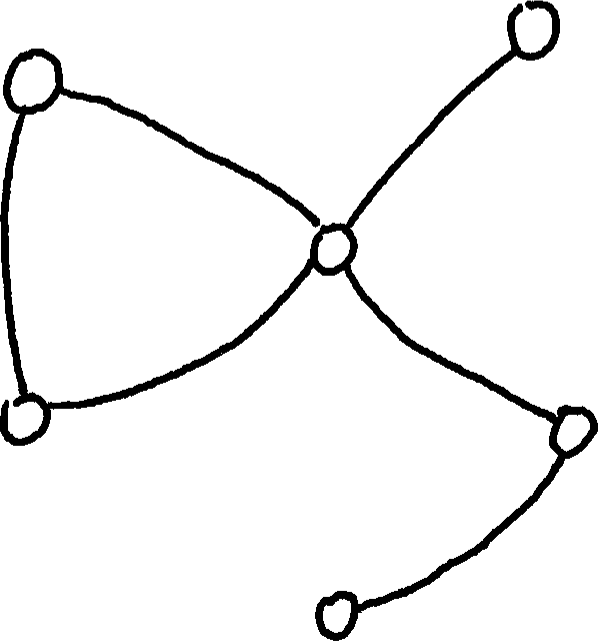
\includegraphics[width=0.3\textwidth]{graphics/L1_exc/unlabeled_simple_graph.png}
  \caption{A simple graph.}
  \label{fig:simple_graph}
\end{figure}

A graph consists, as indicated in Figure \ref{fig:simple_graph}, of \emph{vertices} connected by \emph{edges}. This is the most basic situation we can have, where there are finitely many vertices and each pair of vertices either have an edge between them or not. We will fairly regularly be considering various extensions of this notion, to contain more information. For example, we can add labels to the vertices,\sidenote[][-1cm]{In fact, we will see when we get to the formal definitions that this is probably the most basic notion -- the unlabelled version turns out to be subtler to define.} as in Figure \ref{fig:labelled_simple_graph}.

\begin{figure}
  \centering
  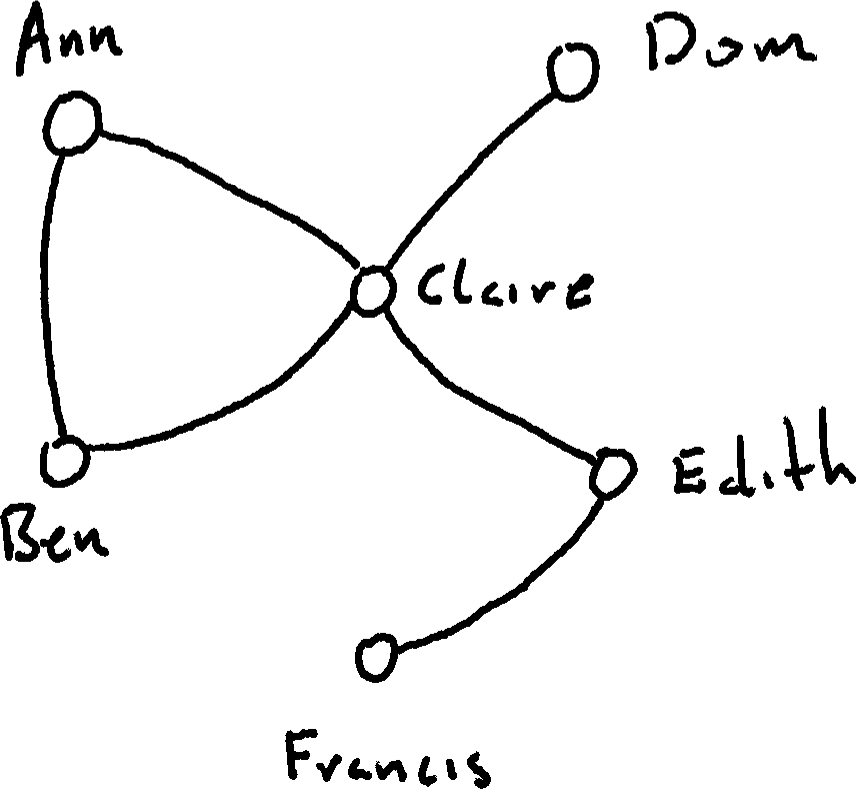
\includegraphics[width=0.3\textwidth]{graphics/L1_exc/labeled_simple_graph.png}
  \caption{A labelled simple graph.}
  \label{fig:labelled_simple_graph}
\end{figure}

The labels we added also start to make clear what kind of real-world thing a graph might model -- if we interpret an edge as saying ``these people are friends'', we have a tiny example of a social network represented as a graph.\sidenote[][]{Now imagine in your head what it would look like if vertices were Facebook accounts and edges were ``are friends'' -- a much larger graph, but an example of the same thing. What might be interesting questions to ask about this graph?

This interpretation of vertices as people and edges as friendships will be common throughout the course, because it is natural given my research interests, and it is an easy down-to-earth example.}

It's not only the vertices we can write things on -- often it is interesting to give each edge a number, called its \emph{weight}, like in Figure \ref{fig:weighted_graph}. Maybe the numbers represent how many hours per day they spend together.

\begin{figure}
  \centering
  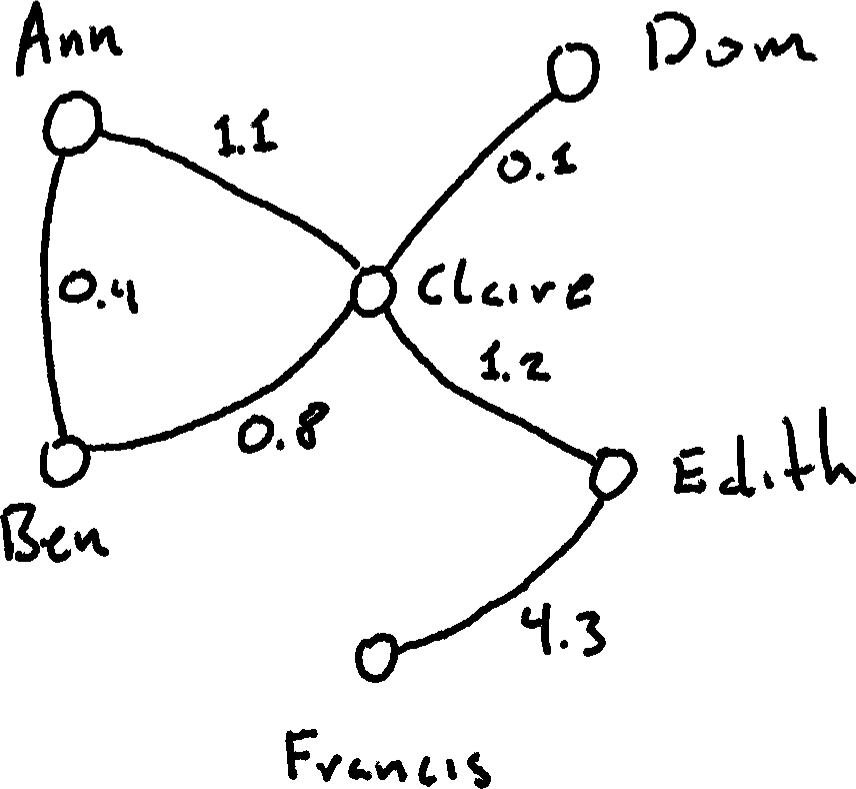
\includegraphics[width=0.3\textwidth]{graphics/L1_exc/weighted_graph.png}
  \caption{A weighted graph.}
  \label{fig:weighted_graph}
\end{figure}

Another common version is to permit multiple edges between vertices, as in Figure \ref{fig:labelled_multigraph}. Perhaps each edge represents a class the two people have in common, so it makes sense to have more than one edge?\sidenote[][-1.5cm]{If you think about it, this is similar to just labelling a single edge with an integer saying how many classes they have in common. However, it has a very different feeling, and the maths we do on multigraphs will be quite different from what we do on weighted graphs.}

\begin{figure}
  \centering
  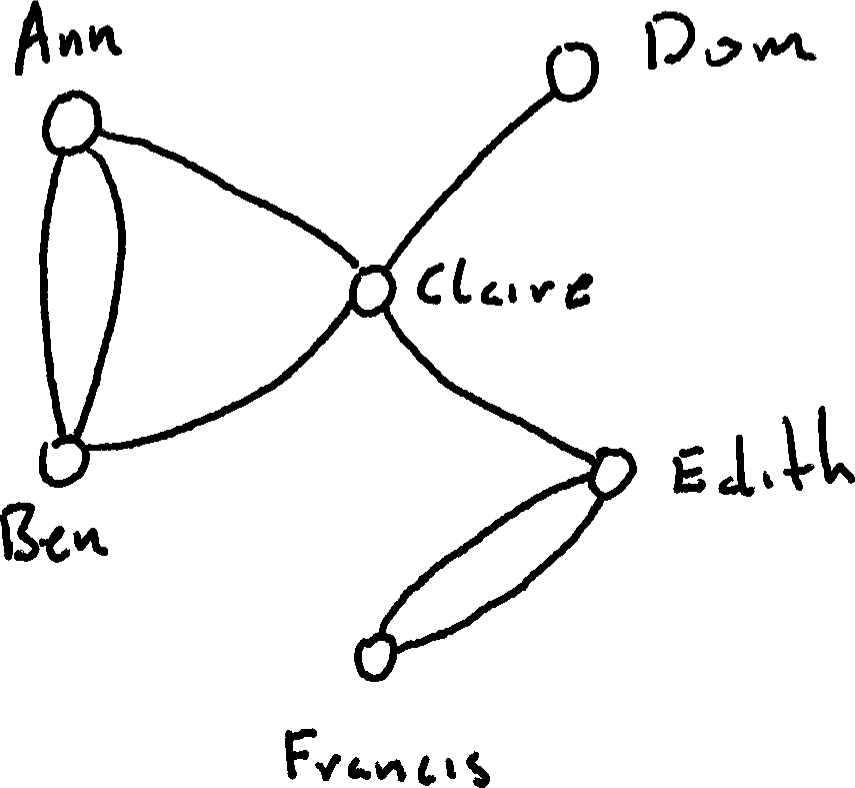
\includegraphics[width=0.3\textwidth]{graphics/L1_exc/multigraph.png}
  \caption[][1cm]{A labelled multigraph.}
  \label{fig:labelled_multigraph}
\end{figure}

Or perhaps the edges have a direction, as in Figure \ref{fig:labelled_digraph}? Now the interpretation might be that an edge means ``is in love with''.\sidenote[][-0.5cm]{So in our figure there is quite a bit of unrequited love and confused emotions -- though perhaps Edith and Francis will find happiness?}

\begin{figure}
  \centering
  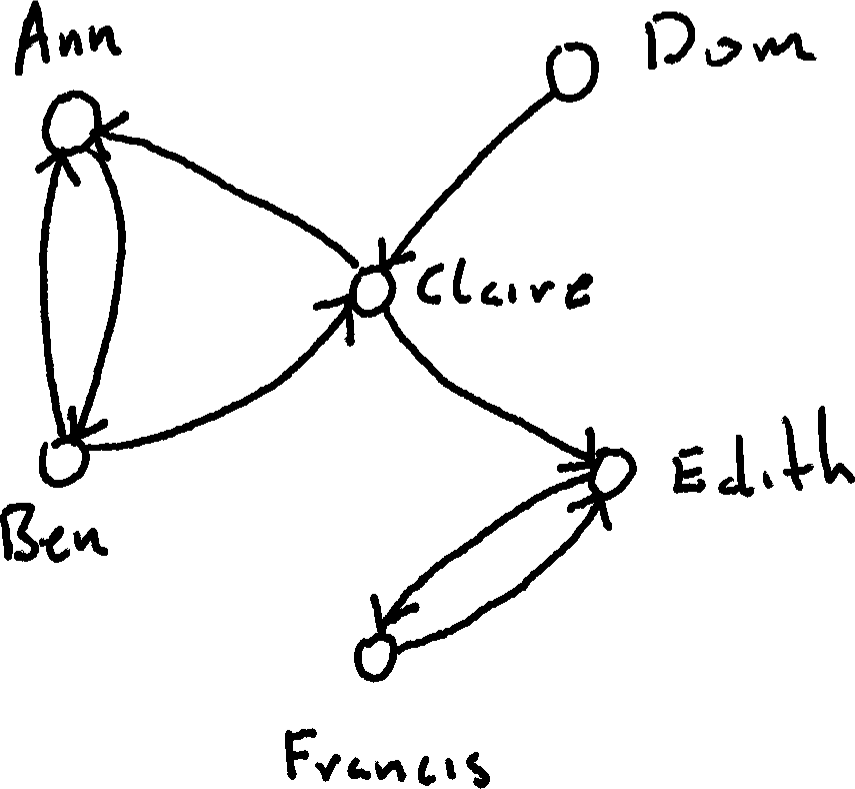
\includegraphics[width=0.3\textwidth]{graphics/L1_exc/digraph.png}
  \caption[][0.8cm]{A directed graph.}
  \label{fig:labelled_digraph}
\end{figure}

The final version that we will actually see used in the course is to give the vertices (or the edges) colours, as in Figure \ref{fig:vertex_coloured_graph}. Now the colour might represent the gender of a person, or some other classification of vertices into various types.

\begin{figure}
  \centering
  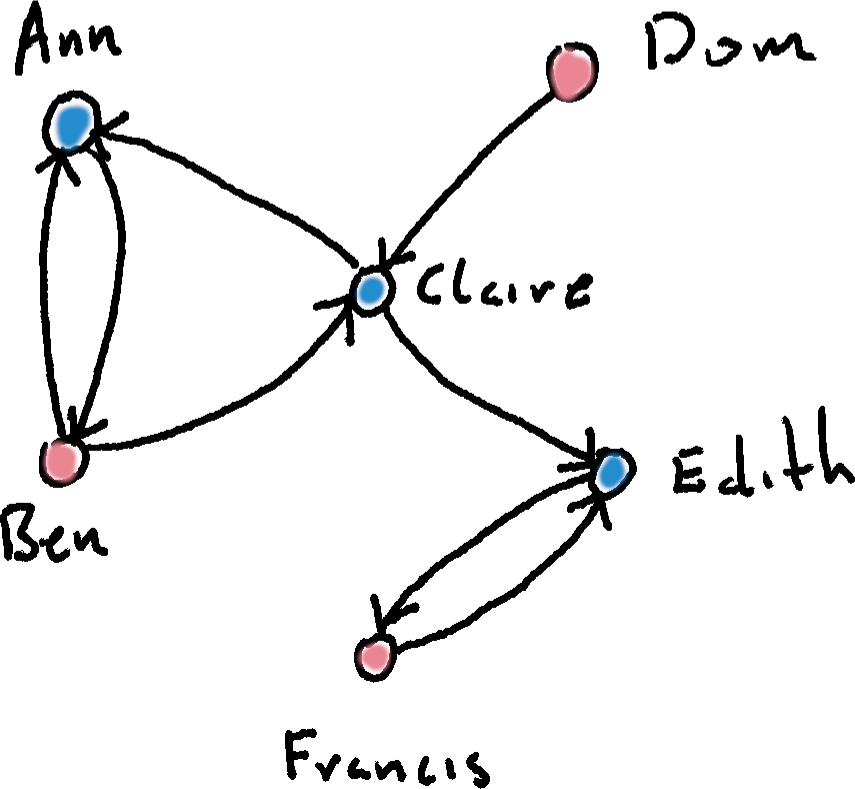
\includegraphics[width=0.3\textwidth]{graphics/L1_exc/vertex_coloured_digraph.png}
  \caption{A directed graph with a vertex colouring.}
  \label{fig:vertex_coloured_graph}
\end{figure}

As we proceed in the course, we will of course give precise mathematical definitions of what exactly each of these types of graph is. For today, however, we don't really need those definitions -- the intuitive descriptions will be enough.

\section{Exercise topic 1: Euler in Königsberg}

The very first thing studied in graph theory, in the early eighteenth century, was the bridges of Königsberg. Königsberg -- today Kaliningrad -- is divided into four parts by the river Pregel, and at the time the city had seven bridges, as in Figure \ref{fig:konigsberg_map}.

\begin{figure}
  \centering
  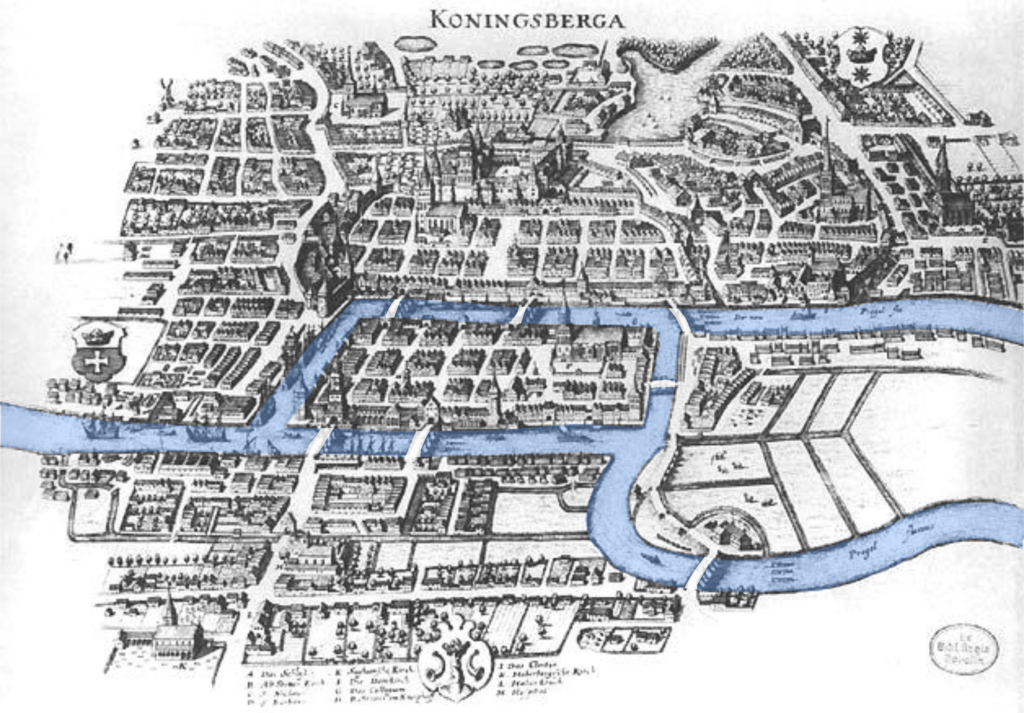
\includegraphics[width=0.9\textwidth]{graphics/L1_exc/konigsberg_map.png}
  \caption{A map of the city of Königsberg.}
  \label{fig:konigsberg_map}
\end{figure}

\begin{xca}
  Can you represent this situation as a graph? Which of the six types of graph we looked at earlier would be most appropriate?
\end{xca}

One question the people of this town would ask themselves, for some reason,\sidenote[][]{Presumably they were all very bored all the time, since they didn't have TikTok yet to keep themselves distracted.} was the following: Is it possible to take a walk around town that uses each bridge exactly once, and takes you back to where you started?

\begin{xca}
  Is it? Convince yourselves that it is not by trying to find such a walk. Can you make it possible by adding or removing edges?

  Try to draw some other graphs where it is possible, and ones where it is not -- can you find some pattern? There is a simple rule to when it is possible or not -- can you figure out what it might be?
\end{xca}

The person who originally solved this problem was the great Leonhard Euler -- in the lecture tomorrow we will see a proof of his result.

If you want to continue on with this exercise and try to prove that the pattern you found always holds, do try and please ask for hints if you need one. It might be rather difficult for you to find the right technique, but it could be a productive sort of difficulty. Or move on to the next exercise.

\section{Exercise topic 2: More examples of graphs}

So far our examples of a graph have been tiny, with six people as the vertices and various relationships between them as edges. We have mentioned that this can generalize to much larger collections of people -- but of course the notion of graph is much much broader than just social relations.

\begin{xca}
  Try to think of more things that can be modelled as graphs, of any of the types we have seen.\sidenote[][]{Or perhaps you can think of something to model as another variant of a graph? We gave five examples of extra structure to give to a graph, but that list was by no means exclusive -- you can come up with new things if you find something new to model.} Try to make your examples as different from each other as possible -- can you think of an example from biology? From finance? From something else you've studied or from one of your hobbies?
\end{xca}

Let us now have a look at a thing we can model using graphs that is of a very different nature from most of the examples we've thought of so far. They've probably all, or nearly all, been of the type ``we go out into the world and measure it'', whether the thing we measure is friendships or debts -- this example is instead a case of a graph arising from some simple rules of a game.

In particular, the game we want to study is the Towers of Hanoi, as illustrated in Figure \ref{fig:towers_of_hanoi}. We have three pegs, labelled $a$, $b$, and $c$, and we have $n$ bricks of increasing size. The bricks must always be in ascending order on every peg, so we can never have a wider brick on top of a narrower brick in the figure. They start in order on peg $a$.

\begin{figure}
  \centering
  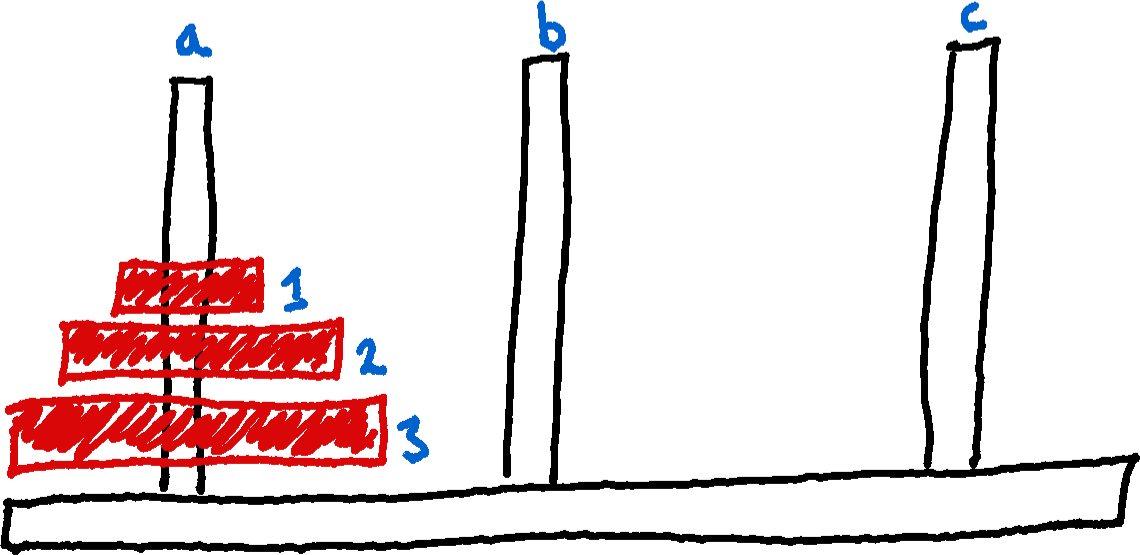
\includegraphics[width=0.6\textwidth]{graphics/L1_exc/towers_of_hanoi.png}
  \caption[][0cm]{The starting state of the Towers of Hanoi, in the $n=3$ case.}
  \label{fig:towers_of_hanoi}
\end{figure}

You are allowed to move the top brick on one peg to a different one, as long as you don't put it on top of a brick with a lower number than itself, i.e. as long as you follow the rule about being narrower than the brick below. The goal of the game is to have all the bricks sitting on peg $c$.\sidenote[][]{In the same order as they were at the beginning on peg $a$, since that is the only order they are allowed to be in by the rules of the game.}

\begin{xca}
  Consider the graph whose vertices are \emph{states} of this game -- so Figure \ref{fig:towers_of_hanoi} represents one vertex, and the state where brick $1$ is on peg $a$ and bricks $2$ and $3$ are on peg $b$ is another vertex. There is an edge between two vertices if you can get between them in a single move. Draw this graph for the small cases of $n=1, 2, 3$.\sidenote[][]{It may be helpful to actually ``make'' this game out of some pieces of paper, drawing the pegs on one and making bricks out of pieces of paper of various size. Getting to play around with it really builds intuition sometimes.}

  Do you see the pattern of what it will look like for larger $n$? Can you write down a formula in terms of $n$ for the minimal number of moves needed to win the game in the general case?
\end{xca}

\section{Exercise topic 3: Same same, but different}

So far we have considered a few different graphs, and answered some questions about them. However, especially to the more algebraically minded, the really interesting thing to study in mathematics is not objects but functions between objects. In this exercise, we will think about functions from one graph to another, and what it means for one graph to be the same as another, or a part of another.

\begin{xca}
  We limit ourselves to considering the case of the labelled simple graphs, like in Figure \ref{fig:labelled_simple_graph}. What might it mean to have a function from one of these graphs to another? Try to think about what might be reasonable, and write down candidate definitions.\sidenote[][-1cm]{The most obvious example of a function you've seen before would probably be one from $\R$ to $\R$ -- but if you've taken a course on algebra before, try to think also of the case of a homomorphism from a group to a group or a ring to a ring.}
\end{xca}

\begin{figure}
  \centering
  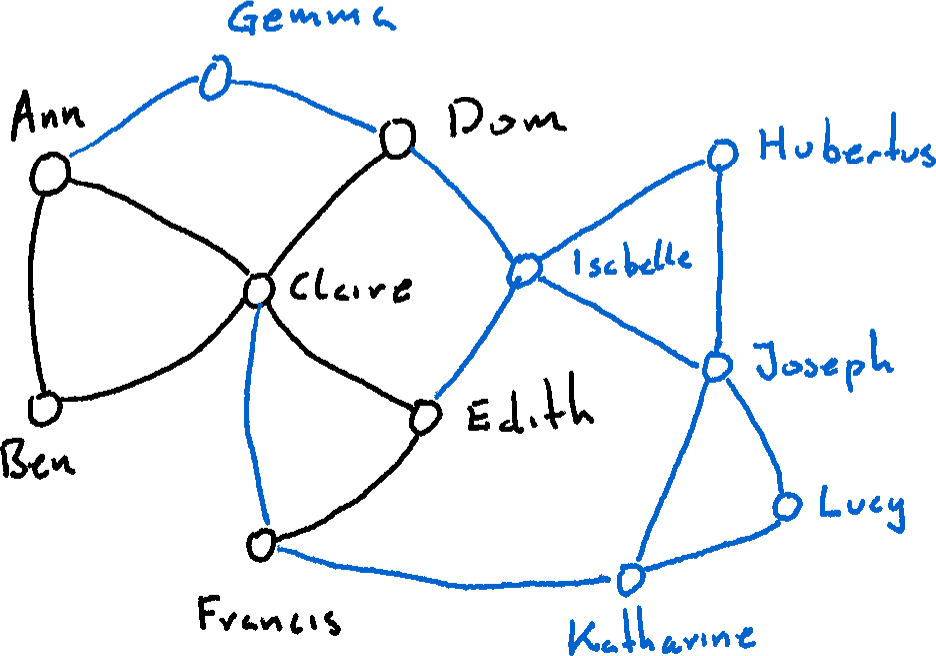
\includegraphics[width=0.8\textwidth]{graphics/L1_exc/subgraph.png}
  \caption[][1cm]{A black subgraph of a larger graph in blue.}
  \label{fig:subgraph}
\end{figure}

\begin{xca}
  Consider Figure \ref{fig:subgraph} -- it should be intuitively clear that what has happened here is that we took the graph from Figure \ref{fig:labelled_simple_graph} and we added some more vertices and more edges. In formal mathematical language, we say that the graph in Figure \ref{fig:labelled_simple_graph} is a \emph{subgraph} of the graph in Figure \ref{fig:subgraph}.

  Can you write a formal definition of what it means for one graph to be a subgraph of another? Perhaps one of your notions of function from one graph to another, or a variation of one, could be useful for this.
\end{xca}

\begin{figure}
  \centering
  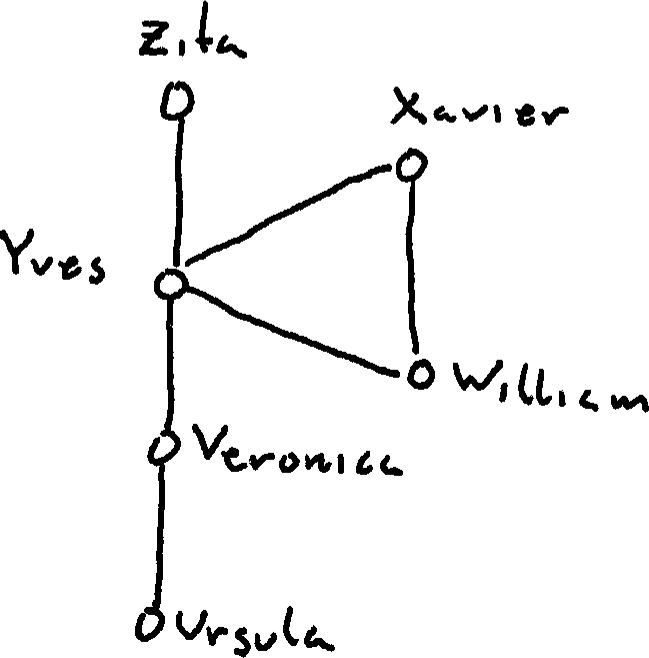
\includegraphics[width=0.4\textwidth]{graphics/L1_exc/isomorph.png}
  \caption[][0cm]{A graph that is suspiciously similar to one we've already seen.}
  \label{fig:isomorph}
\end{figure}

\begin{xca}
    Consider the graph in Figure \ref{fig:isomorph}, and compare it to the one in Figure \ref{fig:labelled_simple_graph}. At first glance, they look quite different -- but if you squint at them the right way, they are the same graph. Can you articulate the sense in which this is true? The formal name for it is that they are \emph{isomorphic}. Again, what you did in the previous parts of the exercise might be helpful.
\end{xca}

If you want to continue thinking about these things, consider the very first graph we saw without any labels, in Figure \ref{fig:simple_graph}. Can we perhaps define what is meant by such an object using what we've seen in this exercise?\sidenote[][]{If you've seen the term ``equivalence class'' before, you can probably make sense of this. If you haven't, you probably need to look that up first.}

%\bibliography{references}
%\bibliographystyle{plainnat}

\end{document}
